%!TEX root = ./ai-jst.tex
%-------------------------------------------------------------------------------
%                            BAB IV
%               	ANALISAN dan PEMBAHASAN
%-------------------------------------------------------------------------------

\chapter{ANALISA DAN PEMBAHASAN}                

\section{Analisa Kebutuhan Sistem}
 Bagian ini menjelaskan hal-hal yang terkait dengan pengembangan aplikasi sebelum penulisan \emph{source code}.
 \subsection{\emph{Flow Chart}}
 Berikut merupakan gambaran umum bagaimana aplikasi ini berkerja. 
 
 	\begin{figure}[H]
	 	\centering
	 	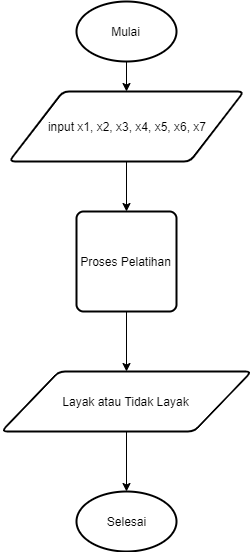
\includegraphics[height=13cm]{gambar/flowchart-jst}
	 	\caption{\emph{Flowchart dari sistem}}
	 	\label{JST-3}
	 \end{figure}
 
 Dimana \emph{input}an x1,x2,x3,x4,x5,x6, dan x7 merupakan variable dari bagian-bagian Tugas Akhir Mahasiswa yang akan lebih dijelaskan pada pembahasan selajutnya.
 
 \subsection{Kebutuhan Kode Sumber \emph{Source Code}}
 Pada pengembangan model jaringan syaraf tiruan ini kami mengunakan sebuah \emph{framework} bahasa pemrograman javascript yaitu Brain.js untuk pemodelan arsitektur JSTnya, sedangkan untuk tampilan kami mengunakan bahasa \emph{markup} HTML dan sebagai \emph{Cascading Stylesheet}nya kami mengunakan pustaka dari materialize css.

\section{Hasil Penelitian}
Data yang kami gunakan didalam penelitian ini merupakan data yang kami dapat dari jurnal yang menjadi titik acuan dan referensi kami \cite{ZeksonArizonaMatondang}.
\subsection{Profil Data}
Data yang dicantumkan pada jurnal yang menjadi referensi kami merupakan data penilaian terhadap Tugas Akhir Mahasiswa yang telah dinormalisasikan dan dibagi menjadi beberapa kriteria sebagaimana tabel berikut.

\begin{center}
	\begin{tabular}{|c|c|c|c|}
		\hline
		No & Variabel & Kriteria \\
		\hline
		1.& x1 & Abstrak \\
		\hline
		2.& x2 & Pendahuluan \\
		\hline
		3.& x3 & Landasan Teori \\
		\hline
		4.& x4 & Metode Penelitian \\
		\hline
		5.& x5 & Hasil dan Pembahasan \\
		\hline
		6.& x6 & Penutup \\
		\hline
		7.& x7 & Daftar Pustaka \\
		\hline
	\end{tabular}
\end{center}
\par 
Data-data yang telah dinormalisasi sebagaimana yang tercantum didalam jurnal terkait bisa dilihat pada tabel berikut.

\begin{center}
	\begin{tabular}{|c|c|c|c|c|c|c|c|c|}
		\hline
		p & x1 & x2 & x3 & x4 & x5 & x6 & x7 & t \\
		\hline
		\hline
		p1 & 0,3 & 0,7 & 0,3 & 0,7 & 0,7 & 0,7 & 0,3 & 1 \\
		\hline
		p2  & 0,7 & 0,7 & 0,7 & 0,7 & 0,9 & 0,7 & 0,7 & 1 \\
		\hline
		p3  & 0,3 & 0,7 & 0,3 & 0,7 & 0,7 & 0,7 & 0,3 & 1 \\
		\hline
		p4  & 0,7 & 0,7 & 0,7 & 0,7 & 0,7 & 0,7 & 0,7 & 1 \\
		\hline
		p5  & 0,3 & 0,7 & 0,7 & 0,9 & 0,7 & 0,7 & 0,7 & 1 \\
		\hline
		p6  & 0,3 & 0,7 & 0,7 & 0,7 & 0,7 & 0,7 & 0,7 & 1 \\
		\hline
		p7  & 0,3 & 0,3 & 0,3 & 0,7 & 0,7 & 0,7 & 0,3 & 0 \\
		\hline
		p8  & 0,7 & 0,3 & 0,7 & 0,7 & 0,7 & 0,7 & 0,3 & 1 \\
		\hline
		p9  & 0,3 & 0,3 & 0,3 & 0,7 & 0,3 & 0,3 & 0,3 & 0 \\
		\hline
		p10 &  0,1 & 0,3 & 0,3 & 0,7 & 0,3 & 0,3 & 0,3 & 0 \\
		\hline
		p11 &  0,3 & 0,3 & 0,7 & 0,7 & 0,7 & 0,7 & 0,7 & 1 \\
		\hline
		p12 &  0,7 & 0,9 & 0,7 & 0,9 & 0,9 & 0,7 & 0,7 & 1 \\
		\hline
		p13 &  0,7 & 0,9 & 0,7 & 0,9 & 0,9 & 0,7 & 0,7 & 1 \\
		\hline
		p14 &  0,3 & 0,3 & 0,7 & 0,7 & 0,7 & 0,7 & 0,3 & 1 \\
		\hline
		p15 &  0,7 & 0,9 & 0,7 & 0,7 & 0,7 & 0,9 & 0,7 & 1 \\
		\hline
		p16 &  0,3 & 0,7 & 0,9 & 0,7 & 0,9 & 0,7 & 0,3 & 1 \\
		\hline
	\end{tabular}
\par
\bigskip
Data latih yang telah dinormalisasikan
\end{center}



\begin{center}
	\begin{tabular}{|c|c|c|c|c|c|c|c|c|}
		\hline
		p36 & 0,7 & 0,7 & 0,7 & 0,7 & 0,9 & 0,7 & 0,7 & 1 \\
		\hline
		p37 & 0,3 & 0,7 & 0,3 & 0,7 & 0,7 & 0,7 & 0,7 & 1 \\
		\hline
		p38 & 0,3 & 0,3 & 0,3 & 0,7 & 0,7 & 0,3 & 0,3 & 0 \\
		\hline
		p39 & 0,7 & 0,7 & 0,7 & 0,9 & 0,7 & 0,7 & 0,7 & 1 \\
		\hline
		p40 & 0,3 & 0,7 & 0,3 & 0,7 & 0,7 & 0,7 & 0,7 & 1 \\
		\hline
		p41 & 0,7 & 0,3 & 0,7 & 0,7 & 0,7 & 0,7 & 0,3 & 1 \\
		\hline
		p42 & 0,7 & 0,7 & 0,7 & 0,7 & 0,9 & 0,7 & 0,7 & 1 \\
		\hline
		p43 & 0,3 & 0,7 & 0,7 & 0,7 & 0,7 & 0,7 & 0,3 & 1 \\
		\hline
		p44 & 0,3 & 0,3 & 0,3 & 0,7 & 0,7 & 0,7 & 0,3 & 0 \\
		\hline
		p45 & 0,3 & 0,7 & 0,7 & 0,7 & 0,7 & 0,7 & 0,7 & 1 \\
		\hline
		p46 & 0,3 & 0,7 & 0,3 & 0,7 & 0,3 & 0,3 & 0,3 & 0 \\
		\hline
		p47 & 0,3 & 0,7 & 0,3 & 0,7 & 0,3 & 0,7 & 0,3 & 0 \\
		\hline
		p48 & 0,7 & 0,7 & 0,7 & 0,7 & 0,9 & 0,7 & 0,7 & 1 \\
		\hline
		p49 & 0,3 & 0,7 & 0,7 & 0,7 & 0,3 & 0,7 & 0,7 & 1 \\
		\hline
		p50 & 0,3 & 0,7 & 0,7 & 0,7 & 0,7 & 0,7 & 0,3 & 1 \\
		\hline
	\end{tabular}
	\par
	\bigskip
	Data uji yang telah dinormalisasikan
\end{center}


Dimana p merupakan simbol dari tugas akhir mahasiswa itu sendiri dan t sebagai target, dengan 1 merupakan untuk kategori layak dan 0 untuk kategori tidak layak.

\subsection{Pembahsan dan Perancangan Arsitektur \emph{Neural Network}}
Metode Jaringan Syaraf Tiruan yang digunakan untuk menilai kelayakan tugas akhir mahasiswa adalah Jaringan Syaraf Tiruan Backpropagation. Metode jaringan syaraf tiruan ini memiliki beberapa lapisan, yaitu lapisan masukan, lapisan keluaran dan beberapa lapisan tersembunyi. Untuk mempermudah pengerjaannya kami mengunakan \emph{framework} jabascript yang memang ditujukan untui pengerjaan arsitektur jaringan syaraf tiruan dengan metode backpropagation yaitu brain.js\footnote{https://brain.js.org}
\par
Arsitektur jaringan syaraf tiruan yang akan kami uji sebagai berikut.
\begin{enumerate}
	\item 7-1-1 (dengan 1 \emph{neuron}).
	\item 7-1-1 (dengan 5 \emph{neuron}).
	\item 7-5-3-1.
	\item 7-3-1.
\end{enumerate} 
Dari hasil \emph{training} dilakukan kepada model JST ini dengan data latih maka didapati hasil sebagai berikut.

\begin{center}
	\begin{tabular}{|c|c|c|c|c|c|c|c|c|}
		\hline
		No & Nilai Error & Jumlah \emph{Hidden Layer} & Jumlah neuron \emph{hidden layer} & \emph{Iteration}  \\
		\hline
		\hline
		1 & 0.00491 & 1 & 1 & 400  \\
		\hline
		2 & 0.00499 & 1 & 5 & 401  \\
		\hline
		3 & 0.00498 & 2 & 8 (5+3) & 433  \\
		\hline
		4 & 0.00497 & 1 & 3 & 388  \\
		\hline
	\end{tabular}
	\par
	\bigskip
	Nilai \emph{error} dan banyaknya \emph{iterasi} untuk masing-masing arsitektur jaringan
\end{center}

\par 
Kami memilih untuk menggunakan arsitektur jaringan ke-4 dimana didapati hasil dari data uji sebagai berikut.

\begin{center}
	\begin{tabular}{|c|c|c|c|c|c|c|c|c|}
		\hline
		No & Target & Hasil Prediksi  \\
		\hline
		\hline
		1 & 1 & 0.995  \\
		\hline
		2 & 1 & 0.960 \\
		\hline
		3 & 0 & 0.260 \\
		\hline
		4 & 1 & 0.891 \\
		\hline
		5 & 1 & 0.976 \\
		\hline
		6 & 1 & 0.953 \\
		\hline
		7 & 1 & 0.966 \\
		\hline
		8 & 0 & 0.341 \\
		\hline
		9 & 1 & 0.917 \\
		\hline
		10 & 0 & 0.516 \\
		\hline
		11 & 0 & 0.257 \\
		\hline
		12 & 1 & 0.910 \\
		\hline
		13 & 1 & 0.876 \\
		\hline
		14 & 1 & 0.967 \\
		\hline
	\end{tabular}
	\par
	\bigskip
	Target dan hasil prediksi untuk masing-masing data uji
\end{center}

\par 
Konsep perhitungan model jaringan syaraf tiruan secara manual yang kami kerjakan dapat disimak pada berikut.
 \begin{enumerate}
 	\item Parameter yang kami gunakan dapat dihitung melalui $ input x jumlah-  \emph{hidden layer} + \emph{Hidden layer} $ dimana \emph{ Hidden layer} dan \emph{output layer} memiliki tambahan \emph{“input”} yang biasa disebut dengan bias. Sehingga didapati $ (7 x 3 + 3) + (3 x 1 + 1) $, sehingga total parameter yang digunakan adalah 28 parameter.
 	
 	\item Memulai  \emph{feedforward training}, kita akan memluai \emph{training} dengan menjumlah setiap \emph{input} dan \emph{weight} di tiap-tiap parameter dimana hal ini bisa dikerjakan dengan $$ j_{n_{in}} = [input x w_{n}] + b_{1} $$
 	
 	\item Nilai yang kita dapati setelah melalui proses diatas akan kita masukkan kedalam \emph{activation function} diaman kita mengunakan \emph{sigmoid} sehingga:
 	$$ Sigmoid(k_{n_{in}}) = \frac{1}{1 + e^{k_{n_{in}}}} $$
 	\item ketika data sudah mengalir ke \emph{neuron} paling akhir \emph{output} kita akan menghitung nilai \emph{error}nya dengan $$ Loss = \frac{1}{2}(output-O_{out})^{2} $$
 	
 	\item Pada tahap ini kita akan memulai aktivitas backpropagation untuk mengubah nilai tiap-tiap \emph{weight} dan bias sehingga kita mendapatkan nilai error yang paling terkecil.
 \end{enumerate}


% Baris ini digunakan untuk membantu dalam melakukan sitasi
% Karena diapit dengan comment, maka baris ini akan diabaikan
% oleh compiler LaTeX.
\begin{comment}
\bibliography{daftar-pustaka}
\end{comment}
